%================ch2======================================
\chapter{Processing the data}\label{ch:ch2}

\section{Collecting Star Cluster Data}
Initially the data from Gaia is queried from the VizieR database \citep{vizier}. The results obtained by Cantat-Gaudin \citep{cg} can be obtained in a tabular form. Hence we obtain the data for 1229 clusters. The database enables us to access position, motion, cataloguing and color information. We require only the photometric data - the color magnitude and the photometric magnitude for the first part. This data was scraped from the website. This enables us to plot a color magnitude diagram for all the clusters. The probablity of being a member was also considered and the clusters with a probability of more than $0.7$ were marked with larger points. The plots of these clusters were analysed, and ten clusters (IC 4651, IC 4756, NGC 752, NGC 1664, NGC 2281, NGC 2287, NGC 2527, NGC 6281, NGC 6405, NGC 6475) were shortlisted for further analysis.

\begin{figure}[h]
	\centering
	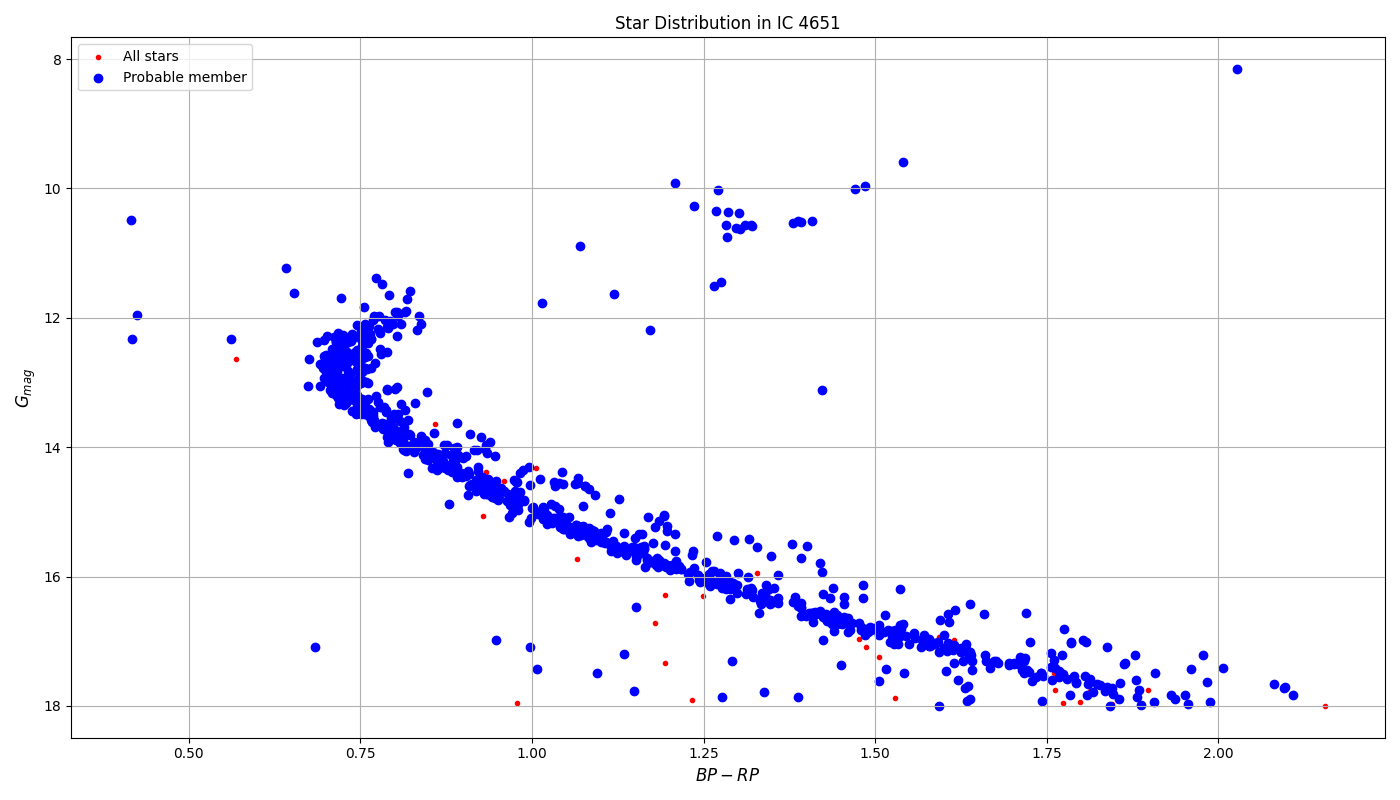
\includegraphics[width=0.8\linewidth]{IC 4651.png}
	\caption{CMD for the cluster IC 4651}
	\label{fig:im2}
\end{figure}

In each of these plots, two tracks can be observed. One is a thick lower track and there is a slightly sparse track above it. These correspond to single stars and stars in a binary system. These were separated and classified into their categories. To separate the two tracks, an isochrone was fitted to each cluster selected. This isochrone was then duplicated and shifted up by a certain value. The stars in between the isochrone and its twin are the single stars and the stars above the twin are the binary stars.

\section{Collecting Isochrone Data}
The data for isochrones is available in the CMD database \citep{cmdSite}. It provides interpolated isochrones. This photometry can be used for studying the clusters we have at hand. We also need distance, metallicity and age to plot the ischrone. This data is available for all clusters in this study from the WEBDA database \citep{webda}, operated by the Department of Theoretical Physics and Astrophysics of the Masaryk University. To plot the cluster data and isochrone together, we need to process the isochrone data. To do this, we must find out the extinction coefficient ($A_g$) for the data. The mean and median value for this is calculated from the downloaded cluster data and varied to find the best fit isochrone. Also found are the mean and median values for $E_{BP-RP}$ from the cluster data. Now, the magnitude data from the isochrones consist of absolute magnitudes. This is converted to apparent magnitudes, so that they can be plotted with the stars. Corrections are made for the color axis and magnitude axis to find the best fit isochrone. Then a shift value is added to the magnitude values of the isochrones' $(x,y)$ pairs so that the binary track can be separated.
$$g_{mag} = G_{mag} + (5 \log(d)) - 5 + A_g$$
$$e_{BP-RP} = G_{BP} - G_{RP} + E_{BP-RP}$$

\begin{figure}[h]
	\centering
	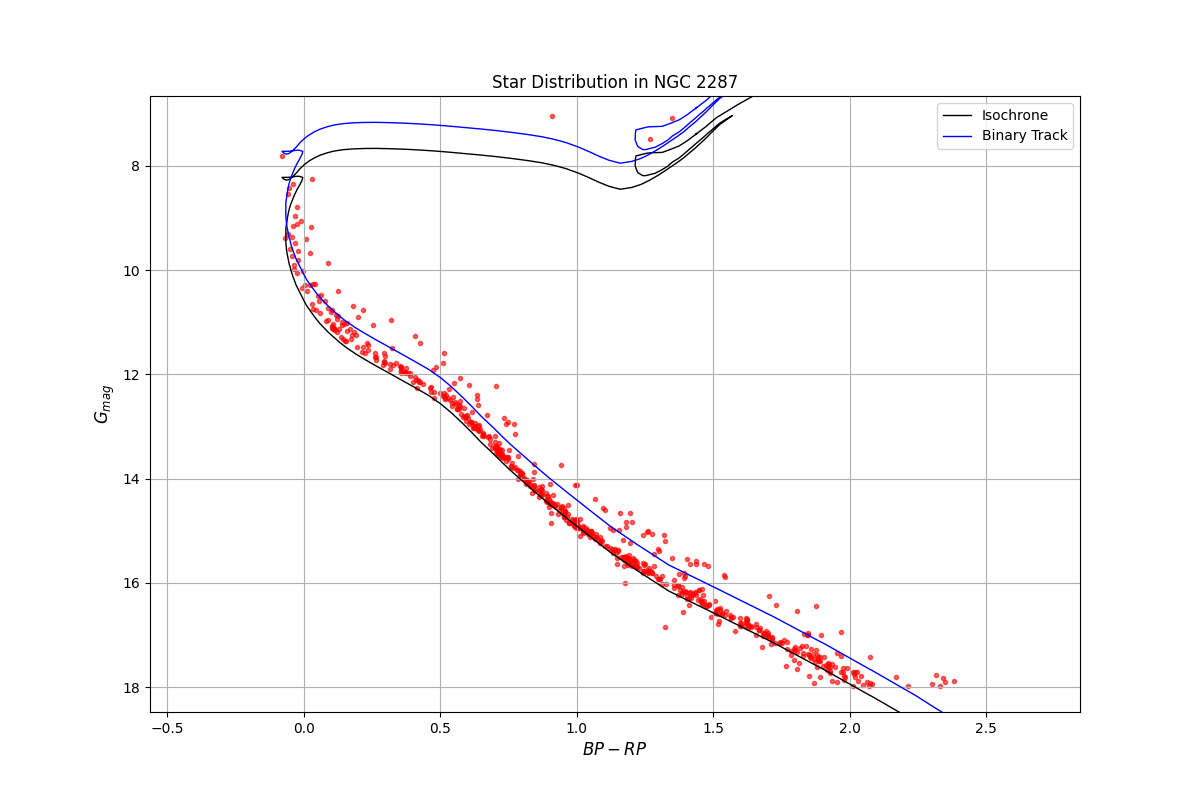
\includegraphics[width=\linewidth]{NGC 2287.png}
	\caption{CMD with isochrone for NGC 2287}
	\label{fig:im3}
\end{figure}


